\chapter{Medida del rendimiento y perfilado}
\label{chap:medida_rendimiento_perfilado}

\lettrine{U}{na} vez expuesta la motivación y habiendo documentado cómo se construye la Prueba de Concepto para la medida de rendimiento en redes densas y dispersas con diferentes implementaciones, en este capítulo se muestran los resultados de estas medidas, tanto para aquellas implementaciones basadas en librerías como para la basada en una arquitectura \textit{point-to-point}. Estos resultados pueden compararse con los que se reportan en la literatura ya existente, comprobando si la red implementada se adhiere a los patrones de \textit{speedup} según dispersión que se pueden observar en la Sección \ref{sec:investigacion_optimizaciones_propuestas}. Por último, se muestran modelos \textit{roofline}\footnote{\url{https://www.intel.com/content/www/us/en/developer/articles/guide/intel-advisor-roofline.html}} de diferentes códigos generados con diferentes compiladores, a modo de comparación en cuanto a la calidad de la generación de código máquina de los mismos.

\section{Metodología}
\label{sec:metodologia}
La medida del rendimiento de la Prueba de Concepto se realiza por secciones, mediante el empleo del reloj del sistema en microsegundos. Dado que los códigos densos y de librería son simples pruebas de concepto, las funciones auxiliares como por ejemplo \texttt{map\_and\_bias} no están debidamente paralelizadas con \texttt{OpenMP}, a diferencia de la versión \textit{point-to-point}, donde su paralelización es tarea trivial teniendo en cuenta que \texttt{OpenMP} ya es necesario para su funcionamiento base. Si bien implementar soporte para \texttt{OpenMP} en los programas de librería no es difícil, ya que esto consistiría en hacer un \textit{backport} del código paralelo de la versión \textit{point-to-point}, parece innecesario cuando el objetivo es medir las posibilidades de una aproximación, centrándose en el producto de matrices, y no tanto el optimizar y trabajar a fondo con una implementación de prueba empleada únicamente como contraste.

Por esta razón, se ha decidido implementar de forma sencilla la generación de código con las librerías \texttt{OpenBLAS} y \texttt{librsb} sin el empleo de \texttt{OpenMP}, pero sin embargo paralelizar al completo la versión \textit{point-to-point}. El procesado auxiliar de datos de forma secuencial, como por ejemplo el que realiza la función \texttt{map\_and\_bias} para los códigos con funciones de librería, representa una porción creciente del tiempo de ejecución conforme las funciones optimizadas de \texttt{OpenBLAS} y \texttt{librsb} tienen acceso a más núcleos de CPU. Sin embargo, debido a que las mediciones de tiempos se realizan de forma aislada, el tiempo extra que representen estas funciones secuenciales no afecta en absoluto a la medida final.

\subsection{Consideraciones generales}
\label{ssec:consideraciones_generales}
Para la medida del rendimiento y perfilado se han generado dos redes neuronales de gran tamaño, una densa con capas completamente conexas de anchos tal que \{capa de entrada, 9 capas ocultas, capa de salida\} = \{24, 500, 800, 1000, 1200, 600, 400, 200, 100, 50, 1\}, y varias redes dispersas basadas en esta primera, con índices de dispersión del 60\%, 70\%, 80\%, 85\%, 90\%, 95\% y 99\%. Estos tamaños no se han seleccionado de forma arbitraria, sino que responden a los índices de dispersión alrededor de los cuales se maximiza el rendimiento y precisión con redes correctamente diseñadas y entrenadas \cite[Figura 4]{hoefler2102sparsity}. Evidentemente, para el problema que se pretende resolver, estas redes están muy sobredimensionadas, siendo en la práctica inútiles en su cometido, puesto que debido a su enorme tamaño, y a la saturación del gradiente que se consigue mediante el uso de la función de transferencia sigmoide, lo único que aprenden durante el proceso de entrenamiento es a marcar como positivos todos los \textit{inputs}.

Esto, que para un ingeniero en inteligencia artificial no posee utilidad práctica, en cuanto a la medida del rendimiento del proceso de inferencia es algo completamente indiferente, ya que, a pesar de la inutilidad de la red creada, esta sigue realizando las cargas de trabajo típicas de una red neuronal adecuada. Esto es, la red tiene que multiplicar matrices, sumar los \textit{bias} y aplicar las funciones de transferencia.

En todas las ejecuciones se han empleado los mismos datos de entrada, basados en el fichero \texttt{input.txt} generado con la función tratada en el punto 3 de la Sección \ref{ssec:extraccion_valores}. En concreto, estos datos exportados se replican 100 y 1000 veces, para obtener un total de $1000 \times 100 = 100000$ y $1000 \times 1000 = 1000000$ datos de entrada.

\subsection{Medida del rendimiento}
\label{ssec:medida_rendimiento_metodologia}
Para la medida del rendimiento se lee el reloj monotónico del sistema empleando la función \texttt{clock\_gettime(CLOCK\_MONOTONIC\_RAW, \&timestamp)}, mediante la cual se miden los tiempos en un total de cinco ejecuciones para compilaciones de \textit{release} (opción \texttt{-s} o \textit{strip}). De estas cinco ejecuciones por cada red e índice de dispersión, se guarda la salida de \texttt{stdout} con el script \texttt{run\_tests.sh}\footnote{Este script también se puede encontrar bajo la carpeta \texttt{res/scripts/} en la raíz del proyecto}:\medskip
\begin{lstlisting}[language=bash]
#!/bin/sh
mkdir -p logs
INPUT=inputs/input_long.txt

for it in 1 2 3 4 5; do
./dense.out $INPUT > logs/dense.$it.log
for sp in 60 70 80 85 90 95 99; do
    echo RUNNING LIBRSB FOR $sp% SPARSITY $it ITERATION
    ./sparse_$sp.out $INPUT > logs/sparse_$sp.$it.log

    echo RUNNING P2P FOR $sp% SPARSITY $it ITERATION
    ./p2p_$sp.out $INPUT > logs/p2p_$sp.$it.log
done
done  
\end{lstlisting}

Las ejecuciones para la medición de tiempos se han llevado a cabo en la partición \texttt{compute2} del clúster Plutón\footnote{\url{https://pluton.dec.udc.es/guide/user-guide.pdf}}, cuyas características se muestran en la Tabla \ref{tb:especificaciones_compute2}. Los perfilados, sin embargo, gracias a la similitud de las arquitecturas de CPU entre los equipos, y debido a que el uso de que la última versión de la suite de Intel oneAPI no es posible en los equipos de Plutón, se realizan en un equipo Xiaomi Mi Notebook 15 con las características indicadas en la Tabla \ref{tb:especificaciones_xiaomi}. Las librerías \texttt{OpenBLAS} y \texttt{librsb} han sido compiladas en ambos equipos con las mismas opciones de compilación y versiones de GCC lo más parecidas posible.
\begin{table}[htpb]
\centering
\begin{tabular}{|c|c|}
    \hline
    CPU & 2x Intel Xeon Silver 4216 (2x16C/32T) @ 3.2GHz\\\hline
    RAM & 256GB DDR4 2933Mhz (8 $\times$ 32GB)\\\hline
    S.O. & CentOS Linux release 7.9.2009 (Core) \\\hline
    Kernel & 3.10.0-1160.76.1.el7.x86\_64 \\\hline
    CC & gcc 9.3.0\\\hline
    OpenBLAS & OpenBLAS 0.3.21\\\hline
    librsb & librsb 1.3.0.1\\\hline
\end{tabular}
\caption{\label{tb:especificaciones_compute2}Especificaciones técnicas de un equipo en la partición \texttt{compute2} del clúster Plutón}
\end{table}

\begin{table}[htpb]
\centering
\begin{tabular}{|c|c|}
    \hline
    CPU & 11th Gen Intel Core i7-11370H (4C/8T) @ 3.3GHz\\\hline
    RAM & 16GB DDR4 3200MHz (\textit{Row-of-chips} {\small$\approx$} 2 $\times$ 8GB)\\\hline
    S.O. & Ubuntu 20.04.5 LTS\\\hline
    Kernel & 5.15.0-50-generic \\\hline
    CC & gcc 9.4.0\\\hline
    OpenBLAS & OpenBLAS 0.3.21\\\hline
    librsb & librsb 1.3.0.1\\\hline
    oneAPI & Intel oneAPI 2022.3\\\hline
\end{tabular}
\caption{\label{tb:especificaciones_xiaomi}Especificaciones técnicas del Xiaomi Mi Notebook 15}
\end{table}

\subsection{Análisis y perfilado}
\label{ssec:analisis_perfilado_metodologia}
Para el análisis y perfilado se ha empleado el programa Intel Advisor, el cual permite realizar modelos \textit{roofline} de partes individualizadas de programas, incluyendo las funciones de su librería \acrshort{mkl} (\textit{\acrlong{mkl}}). Esto es especialmente útil para perfilar tanto la implementación densa, que llama a funciones de \texttt{cblas} ampliamente utilizadas, como la \textit{point-to-point}, que no realiza ninguna llamada a librería.

Sin embargo, esta universalidad se pierde con la versión dispersa (\textit{sparse}), ya que se llama a funciones \textit{built-in} de \texttt{OpenBLAS}, así como a funciones propias de \texttt{librsb}, lo que hace que cambiar a la librería \acrshort{mkl} requiera una reprogramación de ciertas líneas del código para poder perfilar las funciones de librería con Intel Advisor. Esta necesidad de reprogramación es algo costoso que inicialmente puede parecer un problema, pero que se puede solucionar sin necesitar trabajo extra al razonar con respecto al modelo \textit{roofline} de la versión densa, tal como se explica en la Subsección \ref{ssec:codigo_sparse_perfilado}.

\subsection{Compilación}
\label{ssec:compilacion_metodologia}
Para compilar las versiones con llamadas a librería, se requiere intercambiar \texttt{OpenBLAS} por la librería Intel \acrshort{mkl} en la versión densa. La versión \textit{point-to-point} no requiere modificaciones significativas ya que únicamente emplea librerías estándar. Para todas las versiones, es necesario desactivar el \textit{stripping} del binario para activar los símbolos de depuración (sustituir parámetro \texttt{-s} por \texttt{-g}). En cuanto a las funciones de \acrshort{blas}, la modificación de las líneas de compilación genéricas que se pueden encontrar en el fichero \texttt{.ipynb} se muestra de forma estructurada a continuación.

\subsubsection{Código denso}
Para la obtención del \textit{roofline model} de la carga de trabajo es necesario, o bien calcularlo manualmente, o bien emplear alguna herramienta adecuada para ello. Como ya se comentó previamente, se emplea Intel Advisor para el perfilado del código, por lo que es necesario compilar el código denso con una configuración que sustituya \texttt{OpenBLAS} por \acrshort{mkl}. Para ello se puede compilar de las siguientes formas:\medskip
\begin{lstlisting}[language=bash]
# Para una compilación convencional sin depuración con OpenBLAS, sería necesario únicamente ejecutar
gcc -march=native -O3 -s common.c dense.c -o dense.out -lm -lopenblas

# Sin embargo, con propósitos de perfilado con Intel Advisor, en un entorno bash donde se haya realizado `source /opt/intel/oneapi/setvar.sh` se ha de compilar con:
gcc -march=native -O3 -g3 -DMKL_ILP64 -m64 -I"${MKLROOT}/include" common.c dense.c -o dense.out -L${MKLROOT}/lib/intel64 -Wl,--no-as-needed -lmkl_intel_ilp64 -lmkl_gnu_thread -lmkl_core -lgomp -lpthread -lm -ldl
\end{lstlisting}

\subsubsection{Código \textit{sparse}}
En este caso, debido al uso de \texttt{librsb} como librería de Sparse \acrshort{blas}, la herramienta Intel Advisor no es capaz de analizar el código de librería ni compilando la misma con flags de \textit{debug}. Como se comentó previamente, una adaptación a la librería Intel MKL, a pesar de no ser imposible, no es conveniente. Por esto mismo, más adelante en este capítulo se estiman el rendimiento y posibilidades de mejora del código disperso, en función de los resultados con respecto al código denso. Para compilar el código para \textit{release}, la línea de compilación es la siguiente:\medskip
\begin{lstlisting}[language=bash]
# Para una compilación convencional sin depuración con OpenBLAS, sería necesario únicamente compilar con:
gcc -march=native -O3 -s common.c dense.c -o sparse.out -lm -lrsb -lopenblas
\end{lstlisting}

\subsubsection{Código \textit{point-to-point} (p2p)}
En este caso solamente se emplean librerías estándar, por lo que, para GCC, en las líneas de compilación simplemente se cambia \texttt{-s} por \texttt{-g3}. Por otro lado, y debido a que en este caso la optimización del compilador sí es algo importante (ya que no se utilizan únicamente funciones de librería), también se emplean los dos compiladores de Intel: el antiguo ICC, y el nuevo ICX, basado en LLVM\footnote{La documentación empleada para la compilación, así como para posibles líneas de optimización futura, está disponible en \url{https://www.intel.com/content/www/us/en/developer/articles/guide/porting-guide-for-icc-users-to-dpcpp-or-icx.html}.}:\medskip
\begin{lstlisting}[language=bash]
# Para una compilación con OpenMP
gcc -march=native -O3 -g3 common.c p2p.c -o p2p.out -lm -fopenmp

# Para una compilación sin OpenMP
gcc -march=native -O3 -g3 common.c p2p.c -o p2p.out -lm -fno-openmp

# Además, para comparación con Intel ICC (Legacy)
icc -xHost -O3 -g3 common.c p2p.c -o p2p.out -lm -qopenmp
# Y con el nuevo compilador ICX basado en LLVM
icx -xhost -O3 -g3 common.c p2p.c -o p2p.out -lm -fiopenmp
\end{lstlisting}

\section{Medida de rendimiento}
\label{sec:medida_rendimiento}
En esta sección se muestra una comparación de rendimiento entre las diferentes implementaciones o \textit{backends} para cada \textit{sparsity} y aproximación usada (\texttt{OpenBLAS}, \texttt{librsb} o p2p), basada en medidas obtenidas según la metodología descrita en la Sección \ref{sec:metodologia}.

En primer lugar, en la Figura \ref{fig:rendimiento_100k} se muestran los resultados de \textit{speedup} para 100k datos de entrada. Este \textit{speedup} se calcula comparando el tiempo empleado en la multiplicación de matrices para cada \textit{sparsity} e implementación con respecto al tiempo obtenido empleando \texttt{OpenBLAS}\footnote{Los datos procesados pueden encontrarse en la raíz del proyecto bajo la carpeta \texttt{res/measurements/data\_speedups.xlsx}, así como en crudo en los ficheros comprimidos junto a este.}, tal que:
\begin{equation}
    S(85\%\textit{p2p}) = t_{\text{MatMul}}(\texttt{\small OpenBLAS})\: /\: t_{\text{MatMul}}(85\%\textit{p2p})\nonumber
    \label{eq:speedup_example}
\end{equation}

En la figura se puede observar cómo la aproximación \textit{point-to-point} supera ampliamente a \texttt{OpenBLAS} a partir de aproximadamente el 87,5\% de \textit{sparsity} (la primera \textit{sparsity} medida en la que se supera ampliamente a \texttt{OpenBLAS} es de un 90\%, siendo este 87,5\% una interpolación), mientras que \texttt{librsb} no es capaz de alcanzar a \texttt{OpenBLAS} en ningún caso, lo que quizás indique que esta librería está enfocada a matrices con un índice de dispersión mayor.

En la Figura \ref{fig:rendimiento_1M} se pueden observar resultados muy similares para 1M datos de entrada, destacando quizás que, acercándose a índices mayores de dispersión, el rendimiento mejora mucho más con respecto a una cantidad de datos inferior. Este comportamiento se puede apreciar más claramente en la Figura \ref{fig:cross_speedup_1M_100k}, donde se analiza el \textit{cross-speedup} entre los resultados visibles en la Figura \ref{fig:rendimiento_100k} y los de la Figura \ref{fig:rendimiento_1M}. Esto es, siendo $XS(A/B)$ el \textit{cross-speedup}, $S(A)$ y $S(B)$ el \textit{speedup} obtenido con $A$ y $B$ datos de entrada, respectivamente, se puede decir que la magnitud que se representa gráficamente se calcula tal que:
\begin{equation}
    XS(1M/100k) = S(1M)\: /\: S(100k)\nonumber
    \label{eq:cross_speedup}
\end{equation}

Así, se puede apreciar que la mejora del \textit{speedup} con un \textit{dataset} 10 veces más grande es cada vez más alta a partir del 90\% de \textit{sparsity} para la implementación \textit{point-to-point}, siendo sin embargo inferior el rendimiento obtenido por \texttt{librsb}.

\begin{figure}[htpb]
\centering
\begin{tikzpicture}
    \begin{axis}[
        xmin = 55, xmax = 105, xlabel=\textit{sparsity},
        ymin = 0.01, ymax=19, ymode=log, log basis y=10, ylabel=\textit{speedup}, yticklabels={PADDING, {0,01}, {0,1}, 1, 10},
        width = \textwidth,
        height = 0.55\textwidth,
        grid=both,
        legend pos=north west,
    ]

    \addplot[udcgray,smooth,very thick,mark=*] coordinates {
        (60,1)
        (70,1)
        (80,1)
        (85,1)
        (90,1)
        (95,1)
        (99,1)
    };
    \addlegendentry{OpenBLAS}
    
    \addplot[ficblue,smooth,very thick,mark=*] coordinates {
        (60,0.042)
        (70,0.055)
        (80,0.074)
        (85,0.094)
        (90,0.127)
        (95,0.204)
        (99,0.511)
    };
    \addlegendentry{librsb}

    \addplot[udcpink,smooth,very thick,mark=*] coordinates {
        (60,0.262)
        (70,0.361)
        (80,0.574)
        (85,0.806)
        (90,1.253)
        (95,2.852)
        (99,9.985)
    };
    \addlegendentry{p2p}

    % Kinda ugly
    % \vasymptote[udcpink]{87.72}
    \end{axis}
\end{tikzpicture}
\caption{\textit{Speedups} según \textit{sparsity} para 100k datos de entrada}
\label{fig:rendimiento_100k}
\end{figure}

\begin{figure}[htpb]
    \centering
    \begin{tikzpicture}
        \begin{axis}[
            xmin = 55, xmax = 105, xlabel=\textit{sparsity},
            ymin = 0.01, ymax=19, ymode=log, log basis y=10, ylabel=\textit{speedup}, yticklabels={PADDING, {0,01}, {0,1}, 1, 10},
            width = \textwidth,
            height = 0.55\textwidth,
            grid=both,
            legend pos=north west,
        ]
    
        \addplot[udcgray,smooth,very thick,mark=*] coordinates {
            (60,1)
            (70,1)
            (80,1)
            (85,1)
            (90,1)
            (95,1)
            (99,1)
        };
        \addlegendentry{OpenBLAS}
        
        \addplot[ficblue,smooth,very thick,mark=*] coordinates {
            (60,0.037)
            (70,0.050)
            (80,0.069)
            (85,0.087)
            (90,0.120)
            (95,0.201)
            (99,0.550)
        };
        \addlegendentry{librsb}
    
        \addplot[udcpink,smooth,very thick,mark=*] coordinates {
            (60,0.289)
            (70,0.399)
            (80,0.629)
            (85,0.850)
            (90,1.367)
            (95,3.352)
            (99,15.694)
        };
        \addlegendentry{p2p}
        \end{axis}
    \end{tikzpicture}
    \caption{\textit{Speedups} según \textit{sparsity} para 1M datos de entrada}
    \label{fig:rendimiento_1M}
\end{figure}

\begin{figure}[htpb]
    \centering
    \begin{tikzpicture}
        \begin{axis}[
            xmin = 55, xmax = 105, xlabel=\textit{sparsity},
            ymin = 0.8, ymax=1.7, ylabel=\textit{cross-speedup},
            width = \textwidth,
            height = 0.55\textwidth,
            grid=both,
            legend pos=north west,
        ]
    
        \addplot[udcgray,smooth,very thick,mark=*] coordinates {
            (60,1)
            (70,1)
            (80,1)
            (85,1)
            (90,1)
            (95,1)
            (99,1)
        };
        \addlegendentry{OpenBLAS}
        
        \addplot[ficblue,smooth,very thick,mark=*] coordinates {
            (60,0.879)
            (70,0.911)
            (80,0.928)
            (85,0.925)
            (90,0.942)
            (95,0.985)
            (99,1.076)
        };
        \addlegendentry{librsb}
    
        \addplot[udcpink,smooth,very thick,mark=*] coordinates {
            (60,1.105)
            (70,1.104)
            (80,1.096)
            (85,1.054)
            (90,1.091)
            (95,1.175)
            (99,1.572)
        };
        \addlegendentry{p2p}
        \end{axis}
    \end{tikzpicture}
    \caption{\textit{Cross-speedup} según \textit{sparsity} para 1M datos de entrada con respecto a 100k}
    \label{fig:cross_speedup_1M_100k}
\end{figure}

\section{Perfilado y \textit{roofline model}}
\label{sec:perfilado_roofline}
En esta sección se muestran las características de cada carga de trabajo (\textit{workload}) con ayuda de la herramienta Intel Advisor, y se razonan los posibles resultados que no se han podido obtener debido a limitaciones en el análisis.

\subsection{Código denso}
\label{ssec:codigo_denso_perfilado}
Los resultados obtenidos para la red neuronal densa son excelentes, tal como se espera de una librería \acrshort{blas} de amplio uso como \texttt{OpenBLAS}. Estos resultados se obtienen además realizando un excelente uso de la memoria caché, y tal como se observa en el modelo \textit{roofline} de la Figura \ref{fig:roofline_dense}, los resultados que obtiene la librería Intel MKL son extrapolables, por similitud en los tiempos, a los de \texttt{OpenBLAS}.

\begin{figure}[h!]
    \centering
    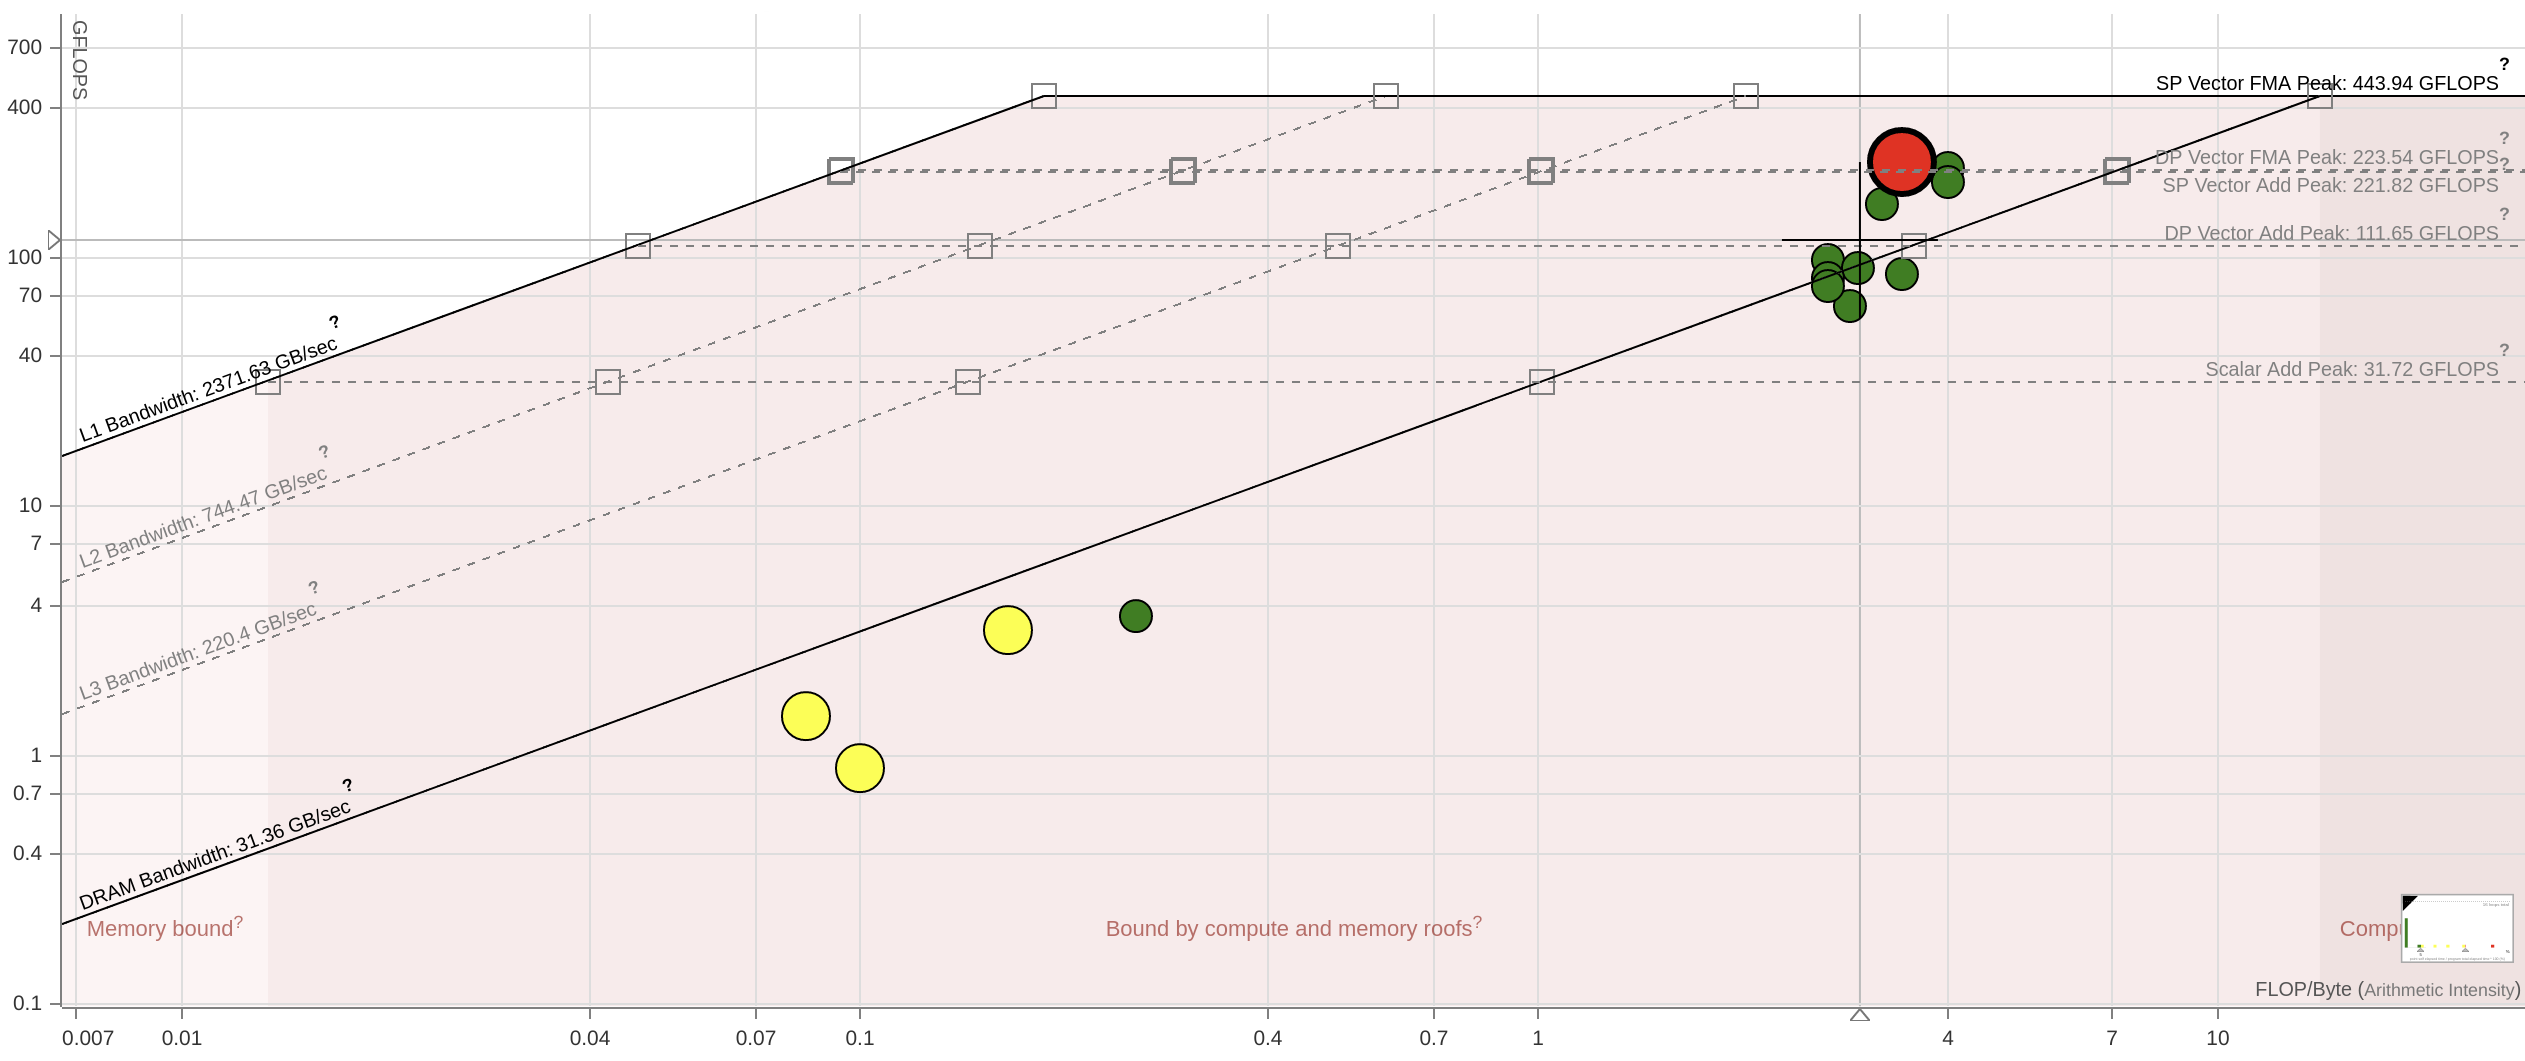
\includegraphics[width=\textwidth]{img/rooflines/roofline_dense.png}
    \caption{\textit{Roofline model} del código denso}
    \label{fig:roofline_dense}
\end{figure}

Como se puede apreciar en el modelo, el \textit{workload} de interés, que es el que se encuentra en la parte superior derecha (coloreado en rojo y verde), corresponde a las funciones \texttt{cblas\_sgemm} (ver punto 2 Subsección \ref{ssec:gdin_matrices_densas}). Estas funciones están fuertemente optimizadas y emplean instrucciones vectoriales AVX512, como se puede observar en los detalles de la carga de trabajo (Figura \ref{fig:roofline_dense_details}).

Fijándose con atención en el modelo, se pueden ver funciones con un desempeño considerablemente inferior en la parte central izquierda (coloreadas en amarillo y verde). Estos puntos corresponden a la función \texttt{map\_and\_bias} y sucesivas llamadas a otras funciones como \texttt{expf}. Como se comentó previamente, una paralelización de funciones auxiliares es sencilla. Sin embargo, y tal como se puede ver en el modelo, se pueden distinguir perfectamente los componentes de dichas funciones, por lo que es sencillo discernir qué mejoras podrían obtenerse mediante una mejora en la eficiencia del producto de matrices.

\begin{figure}[h!]
    \centering
    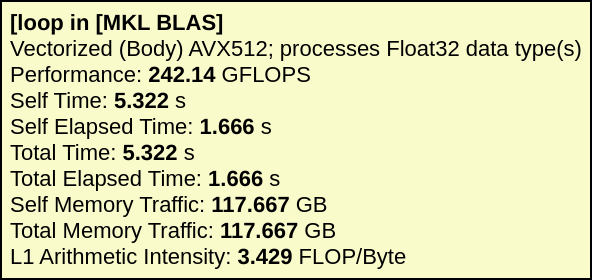
\includegraphics[width=0.5\textwidth]{img/rooflines/roofline_dense_details.png}
    \caption{Detalles de \texttt{cblas\_sgemm} en el modelo del código denso}
    \label{fig:roofline_dense_details}
\end{figure}

\subsection{Código \textit{sparse}}
\label{ssec:codigo_sparse_perfilado}
Por otro lado, los resultados obtenidos para la red neuronal dispersa, y como ya se pudo observar previamente en la Sección \ref{sec:medida_rendimiento}, son algo decepcionantes. En este caso, debido a la utilización de la librería \texttt{librsb}, el modelo \textit{roofline} no contiene información de utilidad (ver Figura \ref{fig:roofline_sparse_details}). Esto, que a todas luces es un problema, deja de serlo teniendo en cuenta que los tiempos de ejecución de una red dispersa al 95\% son 5 veces superiores a los de la red completamente conexa aún teniendo que procesar un 95\% menos de datos. Por tanto, se puede realizar una estimación del número teórico de FLOPs necesarios para las operaciones de multiplicación.

\begin{figure}[h!]
    \centering
    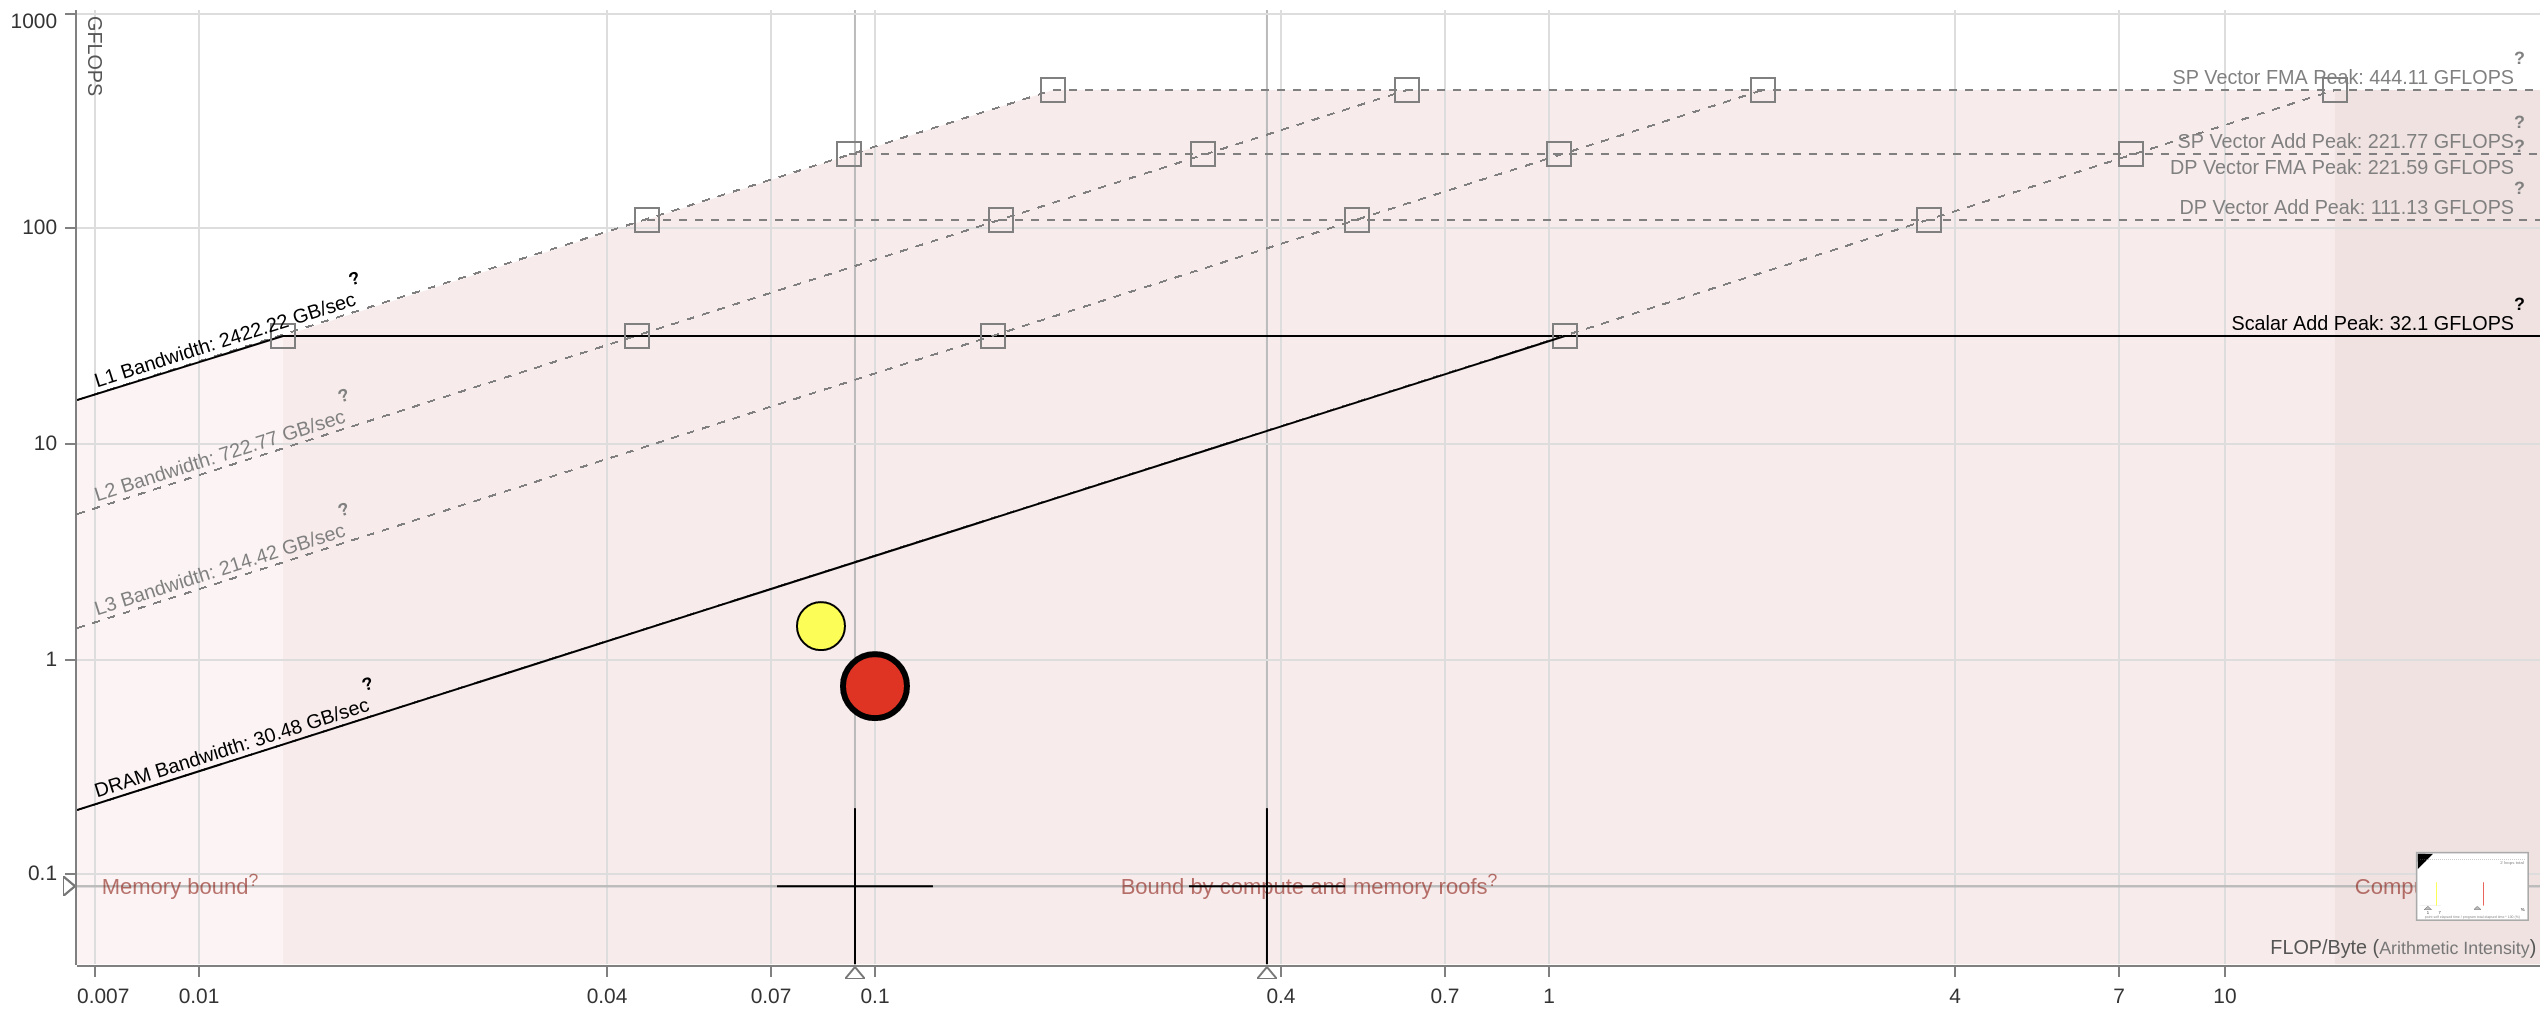
\includegraphics[width=\textwidth]{img/rooflines/roofline_sparse.png}
    \caption{\textit{Roofline model} del código disperso}
    \label{fig:roofline_sparse_details}
\end{figure}

\subsubsection{Aproximación teórica}
Tal como se explica en la Sección \ref{sec:multiplicacion_point_to_point}, teniendo en cuenta que una operación \texttt{\acrshort{fma}} realiza dos FLOPs, se puede concluir que el número de FLOPs para la multiplicación de dos matrices $d\times D$ (de dimensiones $m \times n$ y $n \times k$) será $2 \cdot \#nz \cdot k$.

\subsubsection{Estimación del rendimiento}
Teniendo en cuenta que las matrices dispersas de pesos en el código disperso tienen una densidad del 5\% (o lo que es lo mismo, una \textit{sparsity} del 95\%), desde un punto de vista teórico se puede concluir que se debería realizar un 95\% menos de operaciones en coma flotante.

Esta reducción en el número de operaciones necesarias, debido a múltiples factores como el principio de localidad, estructura interna a la hora de almacenar la matriz, estructuras de control, así como optimizaciones internas de la propia librería, no se corresponde con una disminución del tiempo de ejecución, sino que más bien ocurre todo lo contrario. Esta reducción en el número de FLOPs no parece a primera vista ser causada por un descenso en la intensidad aritmética, puesto que también se cuenta con una cantidad proporcionalmente menor de bytes de datos. Sin embargo, hay que tener en cuenta que para cada valor de cada matriz se cargan como mínimo dos índices enteros que representan su posición, disminuyendo la intensidad aritmética como mínimo a un tercio. Esto implica reducir el valor en el eje $X$ del modelo \textit{roofline} en un factor de 3.

Por otro lado, sabiendo que se lee un 95\% menos de valores en coma flotante, pero que se tarda cinco veces más, esto repercute en un descenso de $5/0{,}05=100$ veces en FLOPs (es decir, un descenso a la centésima parte, o dos órdenes de magnitud, en el eje $Y$).

Por esta razón, el modelo \textit{roofline} resultante, que la herramienta Intel Advisor es incapaz de generar por emplear una librería externa, se estima tal como se puede observar en la Figura \ref{fig:roofline_sparse_estimado}.

\begin{figure}[h!]
    \centering
    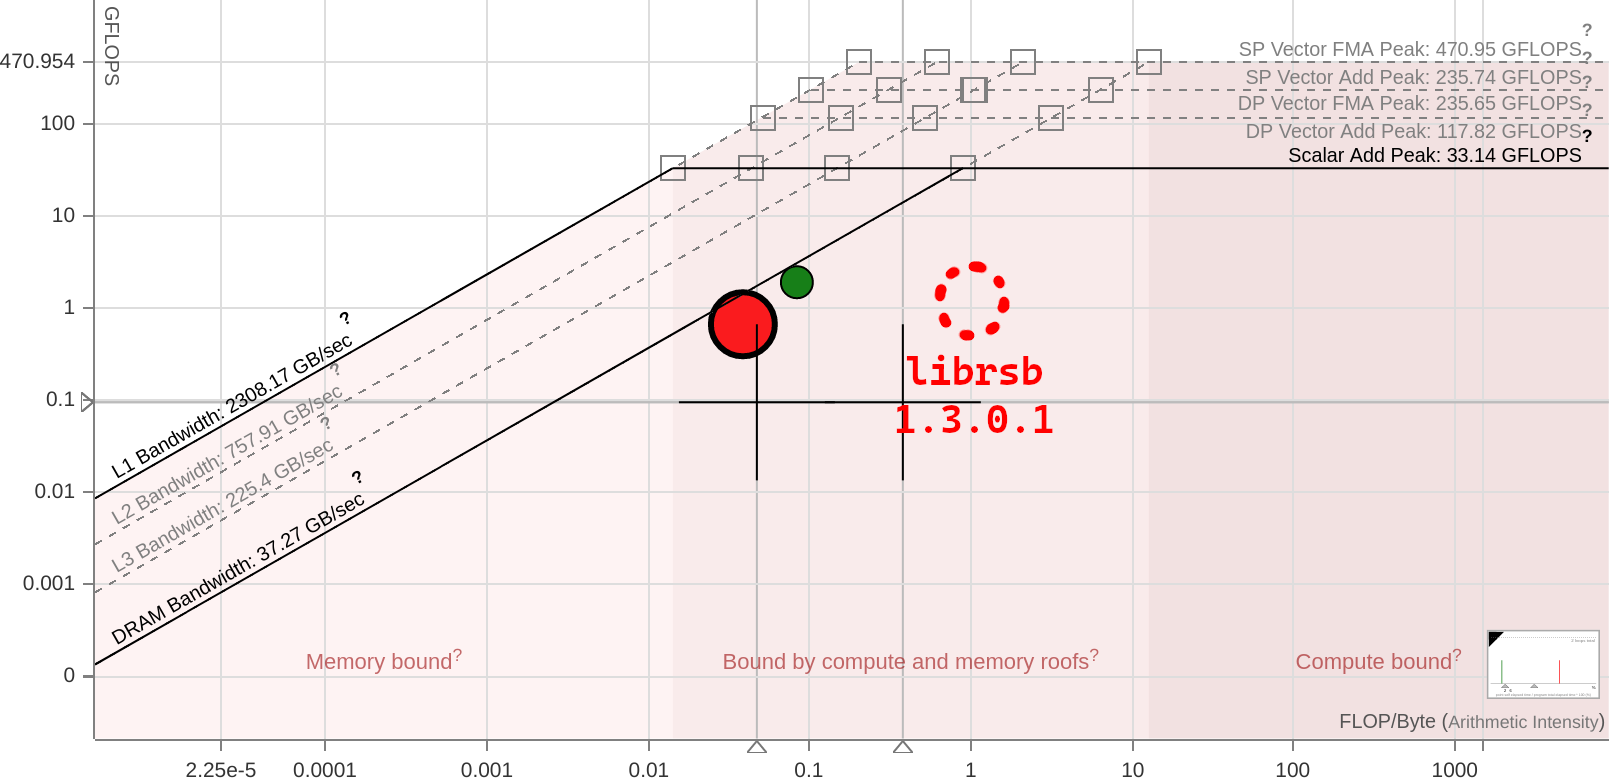
\includegraphics[width=\textwidth]{img/rooflines/roofline_sparse_estimado.png}
    \caption{Estimación del \textit{roofline model} del código disperso}
    \label{fig:roofline_sparse_estimado}
\end{figure}

Estos decepcionantes resultados, sin embargo, motivan la creación de arquitecturas \textit{point-to-point}, ya que implican que existe un amplio margen de mejora mediante el análisis estático de código y la generación de instrucciones \textit{ad hoc}, tanto \texttt{\acrshort{fma}} como de control.


\subsection{Código \textit{point-to-point}}
\label{ssec:codigo_p2p_perfilado}
El código \textit{point-to-point} es mucho más demandante a nivel de caché de instrucciones, así como en análisis estático de código, con tiempos de compilación que se acercan a las 24 horas y decenas de gigabytes de memoria RAM empleada durante el proceso de optimización. Esta aproximación, sin embargo, se espera que tenga un amplio margen de mejora, siendo posible vectorizar y reordenar gran parte de las instrucciones mediante el empleo de la herramienta MACVETH\footnote{\url{https://github.com/UDC-GAC/MACVETH}} \cite{custom_high_performance_vector_codegen_sparse_computations}.

\subsubsection{Compiladores empleados}
Tal como se comentó en la Subsección \ref{ssec:compilacion_metodologia}, para la generación de código \textit{point-to-point} se emplean los compiladores de Intel, ICC e ICX, además del compilador GCC. Debido a que, en este caso, al emplear operaciones estándar de C y no llamadas a librería existe un amplio margen de optimización, resulta interesante observar cómo se comporta GCC al lidiar con diferentes niveles de \textit{sparsity}, así como las diferencias de rendimiento entre los principales compiladores para una \textit{sparsity} fija.

\subsubsection{\textit{Roofline models}}
Para la misma red que en los códigos anteriores, con GCC, se obtiene el modelo que se muestra en la Figura \ref{fig:roofline_p2p_gcc}.
\begin{figure}[h!]
    \centering
    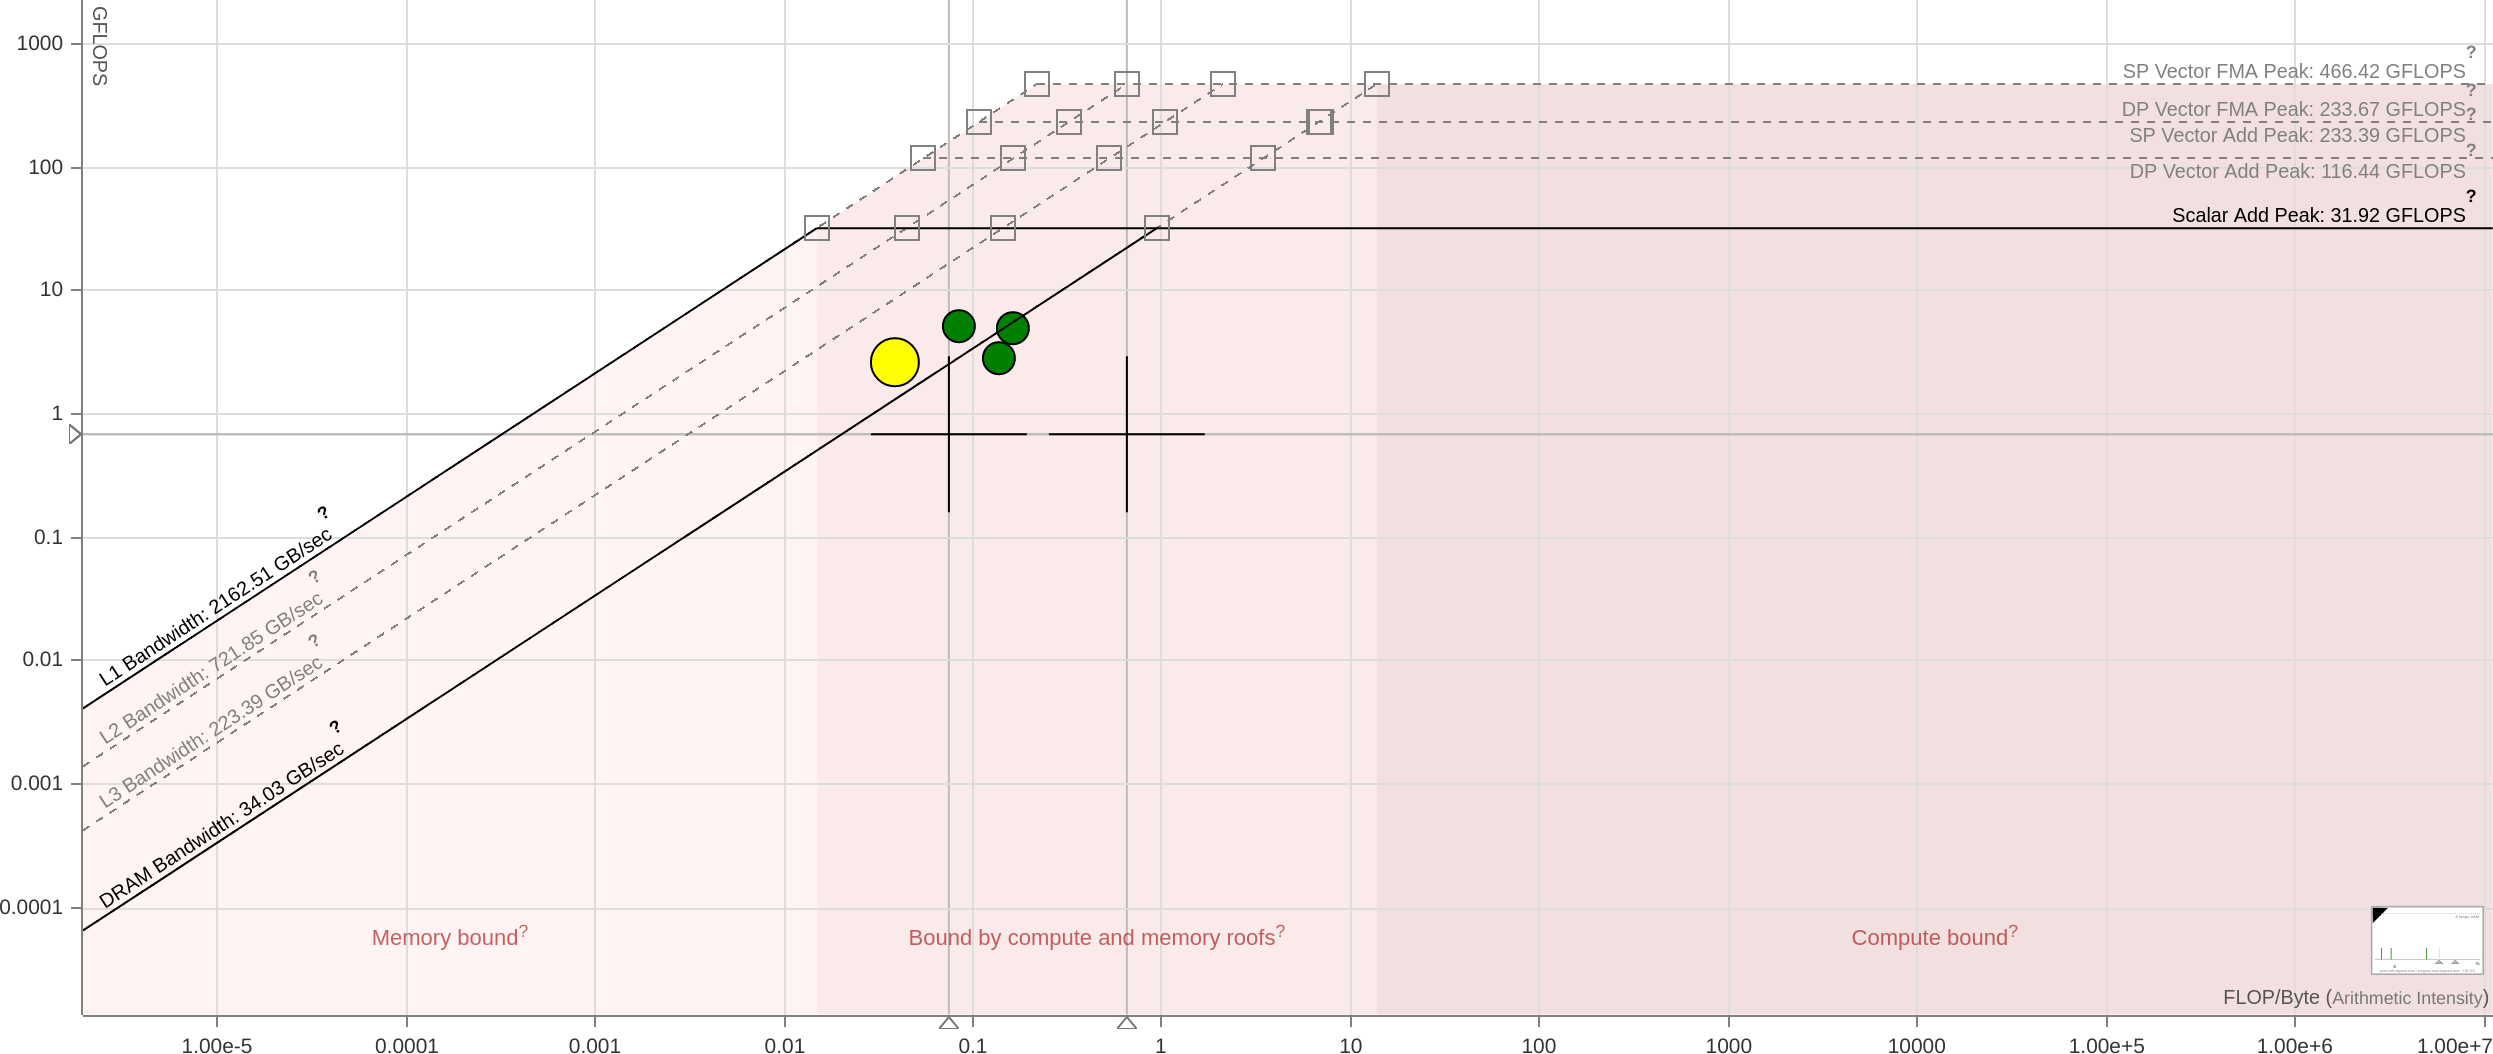
\includegraphics[width=\textwidth]{img/rooflines/roofline_p2p_95.png}
    \caption{\textit{Roofline model} del código \textit{point-to-point} con GCC (95\% de \textit{sparsity})}
    \label{fig:roofline_p2p_gcc}
\end{figure}

Por otro lado, para códigos compilados con GCC, con dispersiones del 90\% y 99\% se obtienen los modelos de la Figura \ref{fig:rooflines_p2p_gcc_90_99}.

\begin{figure}[htpb]
    \centering
    \begin{subfigure}[b]{0.495\textwidth}
        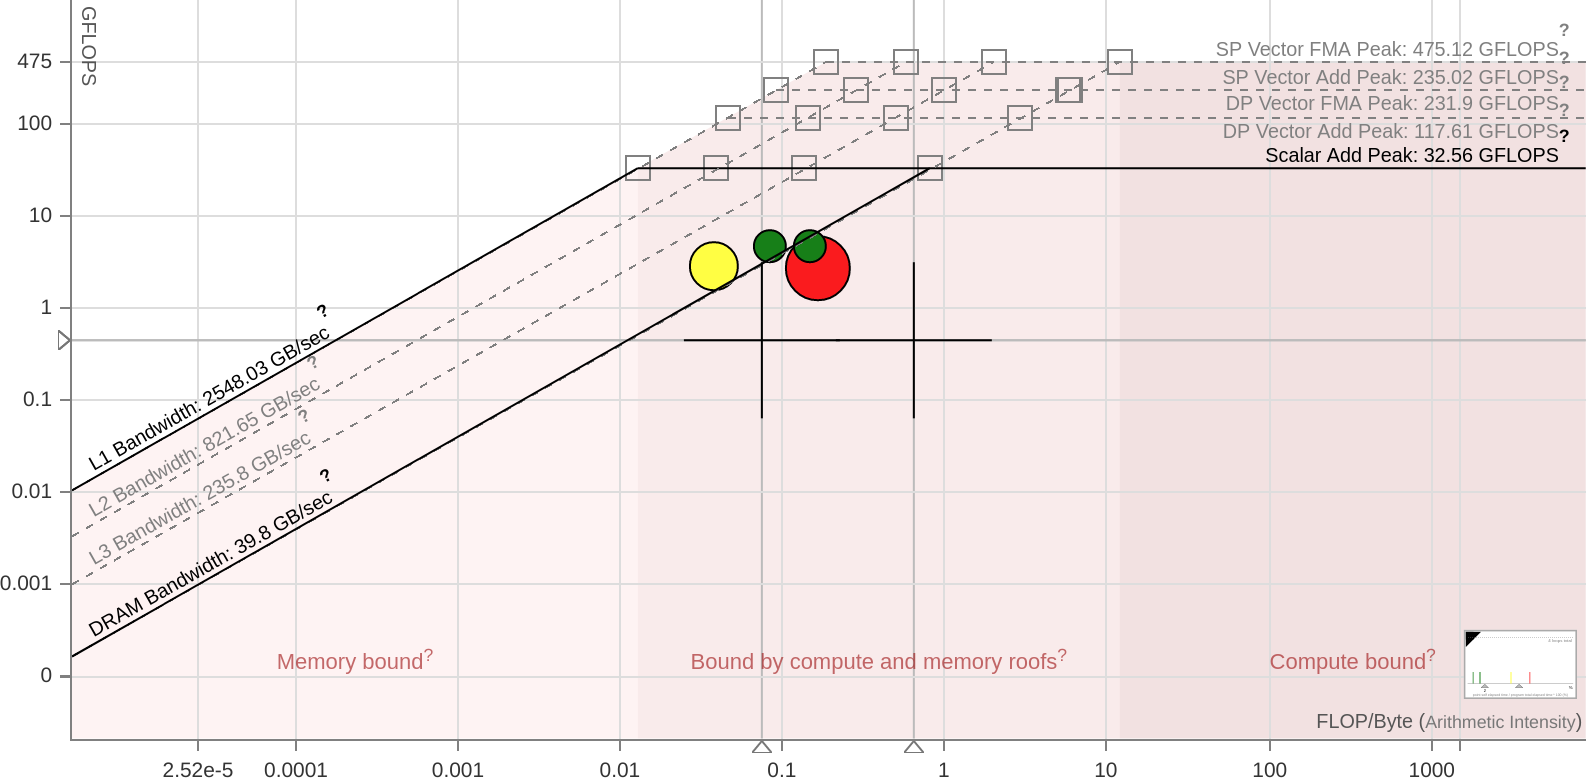
\includegraphics[width=\textwidth]{img/rooflines/roofline_p2p_90.png}
        \caption{\textit{Sparsity} del 90\%}
        \label{fig:roofline_p2p_gcc_90}
    \end{subfigure}
    \begin{subfigure}[b]{0.495\textwidth}
        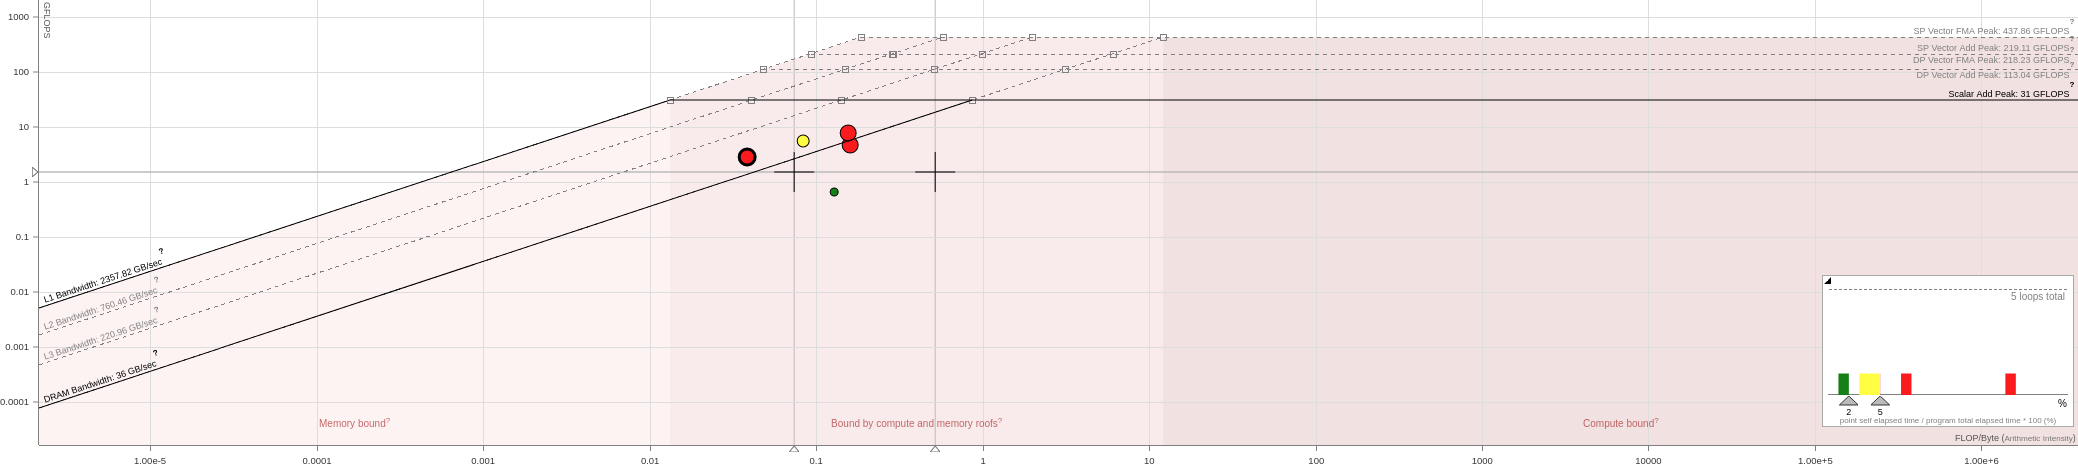
\includegraphics[width=\textwidth]{img/rooflines/roofline_p2p_99.png}
        \caption{\textit{Sparsity} del 99\%}
        \label{fig:roofline_p2p_gcc_99}
    \end{subfigure}

    \caption{\textit{Roofline models} de los códigos \textit{point-to-point} con GCC}
    \label{fig:rooflines_p2p_gcc_90_99}
\end{figure}

Como se puede apreciar, los modelos \textit{roofline} de los códigos \textit{point-to-point} compilados con GCC no son muy diferentes entre ellos, estando todos ellos \textit{memory} y \textit{compute bound}, lo que indica que el código necesita, o bien más ancho de banda a memoria, o bien un patrón de acceso más óptimo, para poder seguir ganando rendimiento a base de potencia bruta de cálculo.

\begin{figure}[htpb]
    \centering
    \begin{subfigure}[b]{0.495\textwidth}
        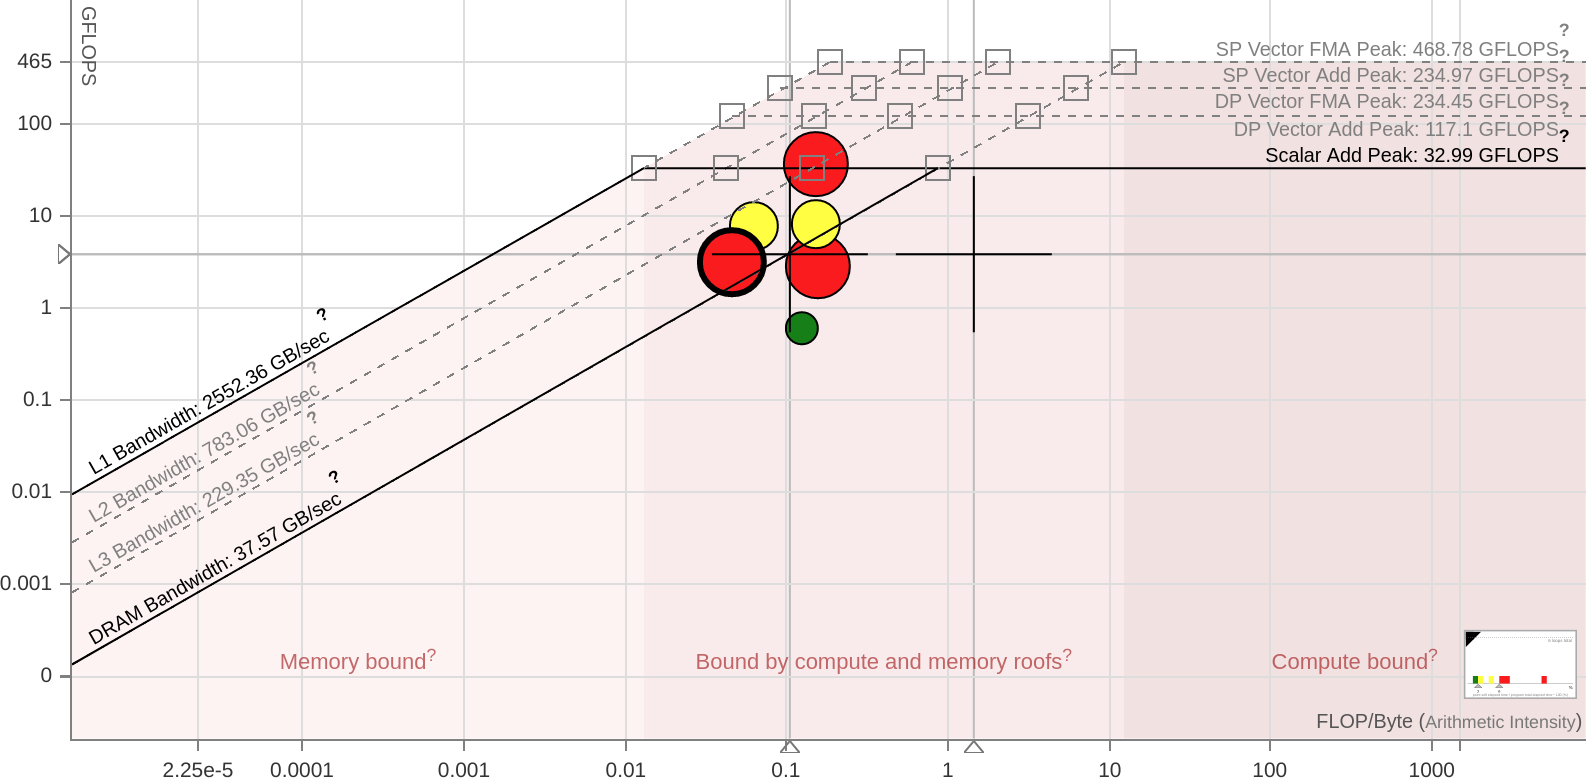
\includegraphics[width=\textwidth]{img/rooflines/roofline_p2p_99_icc.png}
        \caption{ICC}
        \label{fig:roofline_p2p_icc_99}
    \end{subfigure}
    \begin{subfigure}[b]{0.495\textwidth}
        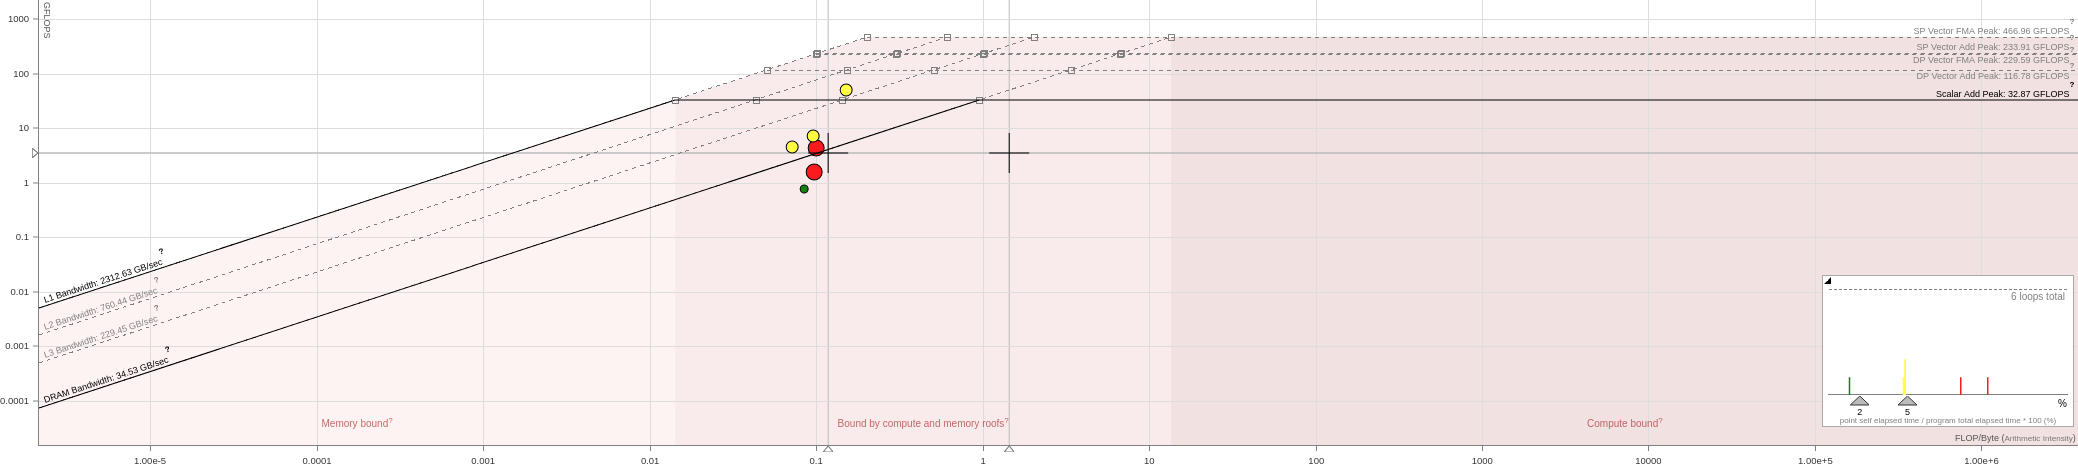
\includegraphics[width=\textwidth]{img/rooflines/roofline_p2p_99_icx.png}
        \caption{ICX}
        \label{fig:roofline_p2p_icx_99}
    \end{subfigure}

    \caption{\textit{Roofline models} de los códigos \textit{point-to-point} con ICC e ICX (\textit{sparsity} del 99\%)}
    \label{fig:rooflines_p2p_icc_icx_99}
\end{figure}

Por último, y como contraste, para las mismas redes al 99\% de \textit{sparsity}, se muestran también los modelos de los códigos compilados con ICC e ICX en la Figura \ref{fig:rooflines_p2p_icc_icx_99}. En este caso, y resultando algo sorprendente, ICC e ICX realizan ambos una optimización muy similar a la de GCC, obteniendo tiempos prácticamente indistinguibles, por lo que a priori no parece obtenerse beneficio con el empleo de estos compiladores. Una diferencia que sí que es importante es que ICX, al estar basado en clang\footnote{\url{https://clang.llvm.org/}}, realiza una compilación mucho más rápida que GCC.

\section{Discusión de los resultados}
Los datos mostrados hasta el momento en este capítulo son cuanto menos sorprendentes. El rendimiento de \texttt{OpenBLAS} es muy bueno, tal como se espera de una librería de dicha importancia. Por otro lado, \texttt{librsb} rinde particularmente mal. Esto indica que quizás esta librería esté orientada a niveles de dispersión varios órdenes de magnitud por encima de los que se utilizan en este trabajo, como por ejemplo para operar con matrices empleadas en redes sociales. Estas contarían con una muy elevada cantidad de ceros antes del primer decimal, que podrían, entre otros, representar a los usuarios que se siguen entre ellos. En este caso, \texttt{librsb} sí que sería particularmente rápida y útil, ya que debido a la naturaleza cambiante de esta clase de matrices, no sería beneficioso generar código \textit{ad hoc} para operar con ellas.

Con respecto a los resultados de los códigos \textit{point-to-point}, los tiempos medidos comienzan a ser mejores que los obtenidos por \texttt{OpenBLAS} por encima de aproximadamente el 87,5\% de dispersión. Si bien esta \textit{sparsity} resulta algo elevada en el ámbito de las redes reuronales y \textit{deep learning} para problemas generales, todavía queda espacio para ganar rendimiento mediante vectorización y optimización de los accesos a memoria, en concreto mejorando la reutilización de la memoria caché y reordenando las operaciones de forma más acertada. Esto puede ser conseguido realizando un correcto filtrado de los datos de entrada, buscando regularidades en los patrones de acceso \cite{piecewise_10.1145/3314221.3314615}, así como mediante el uso de herramientas auxiliares como el previamente citado MACVETH.